% =====================================================================
%  fig-two-approaches.tex  —  editable TikZ source for the Background
%  figure "Two approaches to compliance".
%
%  This is the canonical source for the figure. Colours, type
%  (Source Sans 3), and layout follow the data-viz design system.
%
%  BUILD (writes the vector PDF into ../figures/):
%      pdflatex -output-directory=../figures fig-two-approaches.tex
%      rm -f ../figures/fig-two-approaches.aux ../figures/fig-two-approaches.log
%  The research highlight reads the PDF from ../figures/, so no copy
%  step is needed — rebuild here and re-render the .qmd.
%
%  To edit: change the box labels, headings, or colours below and rebuild.
%  Canvas is 150mm wide; \includegraphics[width=...] scales it to fit.
% =====================================================================
\documentclass[border=0pt]{standalone}
\usepackage[T1]{fontenc}
\usepackage[default]{sourcesanspro}   % same typeface as the document
\renewcommand{\familydefault}{\sfdefault}
\usepackage{microtype}
\usepackage{tikz}
\usetikzlibrary{arrows.meta}

% ---- palette (sampled from the PNG) ---------------------------------
\definecolor{maroon}{HTML}{8A2424}    % title, right column, bottom line
\definecolor{graytext}{HTML}{6F6A63}  % left header, left boxes, arrows
\definecolor{softgray}{HTML}{928D85}  % subtitle + captions (italic)
\definecolor{leftfill}{HTML}{F0EFEC}  % left box fill
\definecolor{rightfill}{HTML}{F7EDEC} % right box fill
\definecolor{rule}{HTML}{DDDDDB}      % divider + bottom rule
\definecolor{ink}{HTML}{333333}       % shared outcome banner (neutral)

\begin{document}
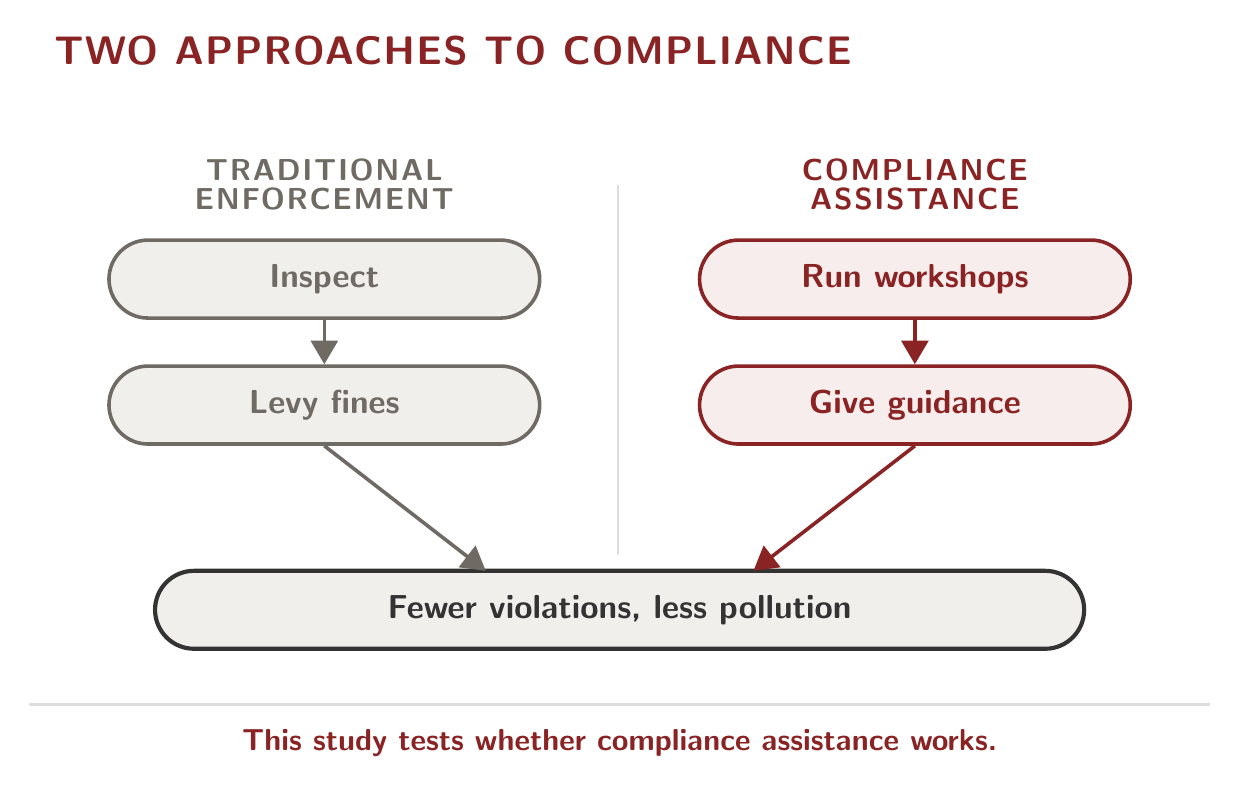
\begin{tikzpicture}[x=1mm,y=1mm,
  box/.style={rounded corners=4.95mm, minimum width=54.7mm,
              minimum height=9.9mm, line width=1.3pt, align=center,
              font=\bfseries\fontsize{11.5pt}{12pt}\selectfont},
  Lbox/.style={box, draw=graytext, fill=leftfill,  text=graytext},
  Rbox/.style={box, draw=maroon,   fill=rightfill, text=maroon},
  Obox/.style={box, minimum width=118mm, line width=1.5pt,
               draw=ink, fill=leftfill, text=ink},
  Larr/.style={graytext, line width=1.3pt, -{Triangle[length=3mm,width=3.4mm]}},
  Rarr/.style={maroon,   line width=1.3pt, -{Triangle[length=3mm,width=3.4mm]}}]

  % --- column + row anchors (mm, y measured up from bottom) ----------
  \def\Lx{37.5}\def\Rx{112.5}
  \def\rowA{68}\def\rowB{52}

  % --- title (top-left) ----------------------------------------------
  \node[anchor=north west, maroon, font=\bfseries\fontsize{14pt}{15pt}\selectfont]
    at (1.9,100.0) {\textls[30]{TWO APPROACHES TO COMPLIANCE}};

  % --- column headers ------------------------------------------------
  \node[graytext, align=center, font=\bfseries\fontsize{10.5pt}{11.5pt}\selectfont]
    at (\Lx,80) {\textls[50]{TRADITIONAL}\\[-0.2ex]\textls[50]{ENFORCEMENT}};
  \node[maroon, align=center, font=\bfseries\fontsize{10.5pt}{11.5pt}\selectfont]
    at (\Rx,80) {\textls[50]{COMPLIANCE}\\[-0.2ex]\textls[50]{ASSISTANCE}};

  % --- left column: traditional enforcement --------------------------
  \node[Lbox] (l1) at (\Lx,\rowA) {Inspect};
  \node[Lbox] (l2) at (\Lx,\rowB) {Levy fines};
  \draw[Larr] (l1.south) -- (l2.north);

  % --- right column: compliance assistance ---------------------------
  \node[Rbox] (r1) at (\Rx,\rowA) {Run workshops};
  \node[Rbox] (r2) at (\Rx,\rowB) {Give guidance};
  \draw[Rarr] (r1.south) -- (r2.north);

  % --- shared outcome banner (both columns converge here) ------------
  \node[Obox] (out) at (75,26) {Fewer violations, less pollution};
  \draw[Larr] (l2.south) -- (58,30.95);
  \draw[Rarr] (r2.south) -- (92,30.95);

  % --- vertical divider (stops above the shared banner) --------------
  \draw[rule, line width=1pt] (74.8,80) -- (74.8,33);

  % --- bottom rule + closing line ------------------------------------
  \draw[rule, line width=1pt] (0,14) -- (150,14);
  \node[anchor=north, maroon, font=\bfseries\fontsize{10.7pt}{12pt}\selectfont]
    at (75,12) {This study tests whether compliance assistance works.};

\end{tikzpicture}
\end{document}
